%%%%%%%%%%%%%%%%%%%%%%%%%%%%%%%%%%%%%%%%%
% Arsclassica Article
% LaTeX Template
% Version 1.1 (10/6/14)
%
% This template has been downloaded from:
% http://www.LaTeXTemplates.com
%
% Original author:
% Lorenzo Pantieri (http://www.lorenzopantieri.net) with extensive modifications by:
% Vel (vel@latextemplates.com)
%
% License:
% CC BY-NC-SA 3.0 (http://creativecommons.org/licenses/by-nc-sa/3.0/)
%
%%%%%%%%%%%%%%%%%%%%%%%%%%%%%%%%%%%%%%%%%

%----------------------------------------------------------------------------------------
%	PACKAGES AND OTHER DOCUMENT CONFIGURATIONS
%----------------------------------------------------------------------------------------

\documentclass[
article,
10pt, % Main document font size
oneside, % One page layout (no page indentation)
BCOR5mm, % Binding correction
]{scrartcl}
\usepackage[a4paper,margin=3cm]{geometry}
\usepackage[italian]{babel}
\usepackage[utf8]{inputenc}
\usepackage{atbegshi}% http://ctan.org/pkg/atbegshi
\usepackage{tikz}
\usetikzlibrary{shapes}
\usepackage{amsmath}
\usepackage{xspace}
\usepackage[usestackEOL]{stackengine}
\usepackage{graphicx}
\usepackage{caption}
\usepackage{subcaption}
\usepackage{float}
\newcommand{\A}{\ensuremath{\mathcal{A}}\xspace}
\newcommand{\B}{\ensuremath{\mathcal{B}}\xspace}
\newcommand\pa[1]{\ensuremath{\left(#1\right)}}
\AtBeginDocument{\AtBeginShipoutNext{\AtBeginShipoutDiscard}}

\hyphenation{Fortran hy-phen-ation} % Specify custom hyphenation points in words with dashes where you would like hyphenation to occur, or alternatively, don't put any dashes in a word to stop hyphenation altogether

%----------------------------------------------------------------------------------------
%	TITLE AND AUTHOR(S)
%----------------------------------------------------------------------------------------

\begin{document}

\begin{center}
\title{
  \begin{figure}[h!]
  \centering
  
\includegraphics[height=2cm,width=5.4cm]{images/WTV_logo.jpg}
  \end{figure}
  WHAT TO VISIT
}
\author{Graziano Grespan 1003760 \\
Carlo Munarini 1050128 \\
Federica Speggiorin 1051031 \\
Sebastiano Valle 1050123}
\end{center} % The article author(s) - author affiliations need to be specified in the AUTHOR AFFILIATIONS block






%\date{} % An optional date to appear under the author(s)

%----------------------------------------------------------------------------------------

%----------------------------------------------------------------------------------------
%	TABLE OF CONTENTS & LISTS OF FIGURES AND TABLES
%----------------------------------------------------------------------------------------

\maketitle % Print the title/author/date block

\setcounter{page}{1} % Set the depth of the table of contents to show sections and subsections only

{\raggedleft\vfill\Longstack[l]{%
Indirizzo: \texttt{http://tecnologie-web.studenti.math.unipd.it/tecweb/$\sim$svalle/homepage.html} \\
Email referente: \texttt{sebastiano.valle@hotmail.it}
}
\raggedright{}
\newpage{}
\tableofcontents % Print the table of contents



\listoffigures % Print the list of figures

\listoftables % Print the list of tables

\section{Abstract}
Il progetto consiste nella realizzazione di un sito Web che presenti ai
visitatori alcune località turistiche suddivise tra località marittime,
località montane e località cittadine.
Gli utenti hanno anche la possibilità di esprimere le proprie opinioni sulle
località esposte aggiungendo dei commenti.

\subsection{Suddivisione ruoli}
Durante il progetto le attività sono state ripartite nel seguente modo:
\begin{itemize}
\item \textbf{Struttura:} Sebastiano Valle, Federica Speggiorin, Graziano Grespan ed in misura minore Carlo Munarini
\item \textbf{Presentazione:} Carlo Munarini, ed in misura minore gli altri componenti
\item \textbf{Front-end:} Graziano Grespan, Sebastiano Valle e Federica Speggiorin
\item \textbf{Back-end:} Sebastiano Valle
\item \textbf{Accessibilità:} Sebastiano Valle, Federica Speggiorin
\item \textbf{Validazione e testing:} Tutti i componenti
\item \textbf{Relazione:} Tutti i componenti
\end{itemize}

\subsection{Schema organizzativo}
Lo schema organizzativo adottato è di tipo ambiguo: sebbene qualche località potrebbe appartenere a più categorie (ad esempio sia città che mare), è stato deciso di associare ad ogni località un'unica categoria per la sua caratteristica di spicco.
Questa scelta è dovuta al fatto che sono previste tre modalità di interazione con il sito:
\begin{enumerate}
\item  l'utente sa già quale località cerca e con la barra di ricerca può direttamente trovare ciò che gli interessa (tiro perfetto nella metafora della pesca), altrimenti nel caso peggiore ha due categorie da esplorare se non trova subito ciò che cerca in una categoria;
\item l'utente ha un'idea precisa del tipo di vacanza che ricerca, ma si aspetta di aumentare le proprie conoscenze riguardo a delle mete di mare/città/montagna durante l'esplorazione del sito (trappola per aragoste nella metafora della pesca);
\item l'utente non sa ciò che cerca ma ha solamente un'idea vaga di ciò che gli interessa; in questo caso, permettendogli di scegliere subito ciò che gli interessa maggiormente, si può far avvertire nell'utente una sensazione di serendipità nell'esplorare nuove località di cui non conosceva nemmeno l'esistenza.
\end{enumerate}
 % 100%

\section{Individuazione degli utenti e delle loro esigenze}\label{sec:requisiti}
Il sito non si pone dei vincoli al target di utenza mirato; in particolare si individuano due macro-categorie di utenti di lingua italiana:
\begin{itemize}
\item L'utente che vuole fare una vacanza e desidera avere più informazioni su
questa, conoscendo già la meta desiderata;
\item L'utente che è alla ricerca di informazioni generiche su una località o
di una vacanza senza conoscerne la meta, navigando senza un obiettivo preciso
all'interno del sito.
\end{itemize}
Si è comunque cercato di rendere accessibile le pagine del sito in modo tale
che questo potesse degradare elegantemente in caso di browser vecchi o testuali
e che il sito fornisse supporti a persone svantaggiate sotto il profilo fisico
o psichico.
Per ogni località sono state individuati dei punti di interesse che sono
ritenuti di notevole attrattiva per il target di utenti scelto, cercando di
includere sia un pubblico giovane che uno più adulto. Tuttavia link esterni che
portano a pagine non in lingua italiana sono stati affiancati da un'indicazione
testuale della lingua in cui è scritta la pagina riferita.
La data, tuttavia, è in formato big-endian (americano AAAA-MM-GG) perchè
l'utenza a cui il sito si rivolge è più che in grado di apprendere facilmente
questo formato, se non è addirittura già conosciuto (a differenza di una
possibile soluzione come middle-endian, ovvero AAAA-GG-MM che potrebbe creare
molta confusione nelle categorie interessate).
 % 100%

\section{Struttura}
Di seguito sono illustrate le modalità di progettazione della struttura delle
pagine all'interno del sito.

\subsection{Parti comuni a tutte le pagine}
Tutte le pagine sono state scritte seguendo lo standard \textit{XHTML 1.0 Strict} e come codifica è stata scelta UTF-8 dal momento che nel sito sono
presenti parole accentate.
Una sezione \textbf{head} ed una sezione \textbf{body} sono state inserite in
tutte le pagine con la stessa struttura.

\subsubsection{Head} %TODO @Graziano @Carlo
Sono presenti i seguenti tag nelle sezioni head di tutte le pagine:
\begin{itemize}
\item \textbf{title:} permette di visualizzare sulla finestra del browser il titolo della pagina visualizzata, dal particolare al generale
\item \textbf{meta title:} indica il titolo della pagina in un eventuale snippet, anch'esso dal particolare al generale
\item \textbf{meta description:} in questo tag viene inserita la breve descrizione della pagina visualizzata in un eventuale snippet
\item \textbf{meta author:} in questo tag sono indicati i componenti del gruppo
\item \textbf{meta keywords:} parole che aiutano un motore di ricerca a trovare la pagina grazie a dei termini di importanza focale
\item \textbf{meta robots:} tag che indica ad un eventuale spider se indicizzare la pagina e se seguire i link da essa uscenti
\item \textbf{meta keywords:} parole che aiutano un motore di ricerca a trovare la pagina grazie a dei termini di importanza focale
\item \textbf{meta reply-to:} %TODO@Graziano
\item \textbf{meta Classification:} tag che serve ad indicare l'argomento trattato dalle pagine del sito
\item \textbf{meta viewport:} %TODO@Carlo
\item \textbf{link shortcut icon:} icona visibile a fianco al titolo della scheda nel browser, aiuta a identificare meglio le schede di \textit{What To Visit} se un utente avesse più schede aperte nel suo browser
\item \textbf{link stylesheet:} collegamento a foglio di stile CSS %TODO@Carlo
\end{itemize}

\subsubsection{Body}
Affinchè l'utente si sentisse il meno disorientato possibile all'interno di \textit{What To Visit}, si è cercato di progettare il sito con un layout essenziale e che mettesse in primo piano il contenuto aspettato in tutte le pagine.
Sono presenti questi elementi strutturali nei corpi di tutte le pagine:
\begin{itemize}
\item un header, dove vi è il logo del sito;
\item un'ampia parte centrale, dove vengono visualizzati i contenuti richiesti dall'utente;
\item un footer, dove sono presenti link ed informazioni di poco rilievo e un'indicazione riguardo la validità della pagina.
\end{itemize}

\subsection{Homepage}
Come pagina principale del sito, si è pensato di esporre in primo piano all'utente la scelta delle tre categorie delle località.
A partire da queste l'utente può arrivare nelle pagine delle categorie, dove può trovare le liste delle località presenti in queste.

Dal momento che la homepage è l'unica pagina facilmente riconoscibile data la sua struttura con tre titoli di indirizzamento, la breadcrumb è stata omessa perchè si è assunto che gli utenti riuscissero a dedurre che si trovano nella homepage quando vi sono dentro (anche grazie all'URL).

Per poter comunque fornire collegamenti alle pagine che non sono di contenuto ma che sono significative (Chi Siamo e F.A.Q.), i link a queste sono stati inseriti nell'header della pagina a fianco del logo; in questo modo, anche se sono di importanza secondaria rispetto ai tre pannelli visualizzati nella pagina, rimangono comunque nella parte visibile del sito quando questo viene aperto (\texttt{http://en.wikipedia.org/wiki/Above\_the\_fold\#In\_web\_design}).

Nel footer, oltre alle indicazioni di validità della pagina, sono stati lasciati i link restanti alle pagine che non sono di contenuto.
 % 100%

\section{Presentazione}\label{sec:presentazione}
In questa sezione vedremo come abbiamo deciso che l'utente debba visualizzare
il nostro sito.

Come anticipato nel punto \ref{sec:struttHead}, ogni pagina può essere
visualizzata in maniera diversa a seconda del dispositivo utilizzato, vi
illustreremo quindi le scelte che abbiamo attuato nelle diverse pagine (I, II,
III Livello) in maniera tale che potessero essere visualizzate nel migliore
dei modi.

Essendo il nostro sito orientato ad un target non specifico che vuole
apprendere informazioni su diverse località, abbiamo deciso di permettere 4
diversi modi di visualizzare la pagina, applicando quindi 4 fogli di stile CSS:
\begin{itemize}
\item \textbf{Foglio di stile \texttt{layout.css}:} questo layout viene
applicato a tutti i dispositivi che visualizzano il nostro sito con più di
780px di larghezza, abbiamo però deciso di ottimizzare tale layout in maniera
che potesse essere accessibile anche a coloro che utilizzano screen-reader
\item \textbf{Foglio di stile \texttt{playout.css}:} una persona che trova
informazioni riguardo ad una località potrebbe decidere scaricare o stampare
il contenuto della nostra pagina così da poterlo guardare in un secondo tempo,
su un PDF od un foglio stampato. Questo stile serve proprio affinchè un utente
possa stampare ogni pagina del nostro sito, visualizzando al meglio le
informazioni chiave della pagina
\item \textbf{Foglio di stile \texttt{tlayout.css}:} questo foglio di stile
entra in gioco quando la pagina viene visualizzata in dispositivi con larghezza
inferiore a 780px. In tal modo il nostro sito offre una visualizzazione pulita
anche su tablet e cellulari
\item \textbf{Foglio di stile \texttt{mlayout.css}:} nel caso What To Visit
venga visualizzato su un cellulare o in una finestra con larghezza inferiore ai
480px, ecco che verrà chiamato in causa questo quarto foglio di stile, molto
simile al precedente, che permette però un eccellente visualizzazione delle
pagine di III livello anche sui cellulari. Il sito è quindi riconosciuto da
Google come \textit{Mobile-Friendly}\footnote{Il \textit{test di compatibilità
con dispositivi mobili} è stato eseguito all'indirizzo:
\texttt{https://www.google.com/webmasters/tools/mobile-friendly/}}
\end{itemize}

\subsection{I colori}\label{sec:Pres-Colore}
Prima di iniziare a guardare nel dettaglio l'aspetto grafico di ogni pagina,
vogliamo presentare quelli che sono i colori adottati nel nostro sito. In What
To Visit infatti gli utenti avranno di fronte a se delle pagine che utilizzano
pochi colori, ai quali abbiamo cercato di attribuire un significato:
\begin{itemize}
\item \textbf{Verde scuro (\#1D653C):} con questo colore, simile ad un verde
primavera scuro, abbiamo voluto indicare gli elementi non attivi ma che
possono essere attivati (come pulsanti per i commenti o i link), gli elementi
fissi della pagina (come footer ed header) oppure elementi non attivabili che
però caratterizzano una località o un collegamento (come succede per indicare
a quale categoria appartiene la località o per indicare un link che non è
stato visitato e porta in una pagina esterna al nostro sito)
\item \textbf{Verde chiaro (\#2ECC71):} Con questa via di mezzo tra un verde
primavera ed un verde smeraldo, si è deciso di indicare quegli elementi che
sono già stati attivati o che potrebbero esserlo poichè puntati dal cursore.
Un esempio possono essere i link già visitati (esterni o interni al sito),
link puntati dal cursore o ancora, i pulsanti per i commenti qualora siano
stati attivati o possano portare al cambiamento/essere frutto di un
cambiamento della pagina
\item \textbf{Grigio Scuro (\#444444):} Questo grigio scuro viene utilizzato
come colore del testo di contenuto e come colore di background per le caselle
di testo nel quale l'utente deve per l'appunto inserire informazioni o commenti
\item \textbf{Bianco (\#FFFFFF):} È presente in tutte le pagine in quanto,
colore di background del sito e della barra di ricerca presente nella
breadcrumb (Vedi punto \ref{sec:IIlev}), unica eccezione riguardante il grigio
scuro come background-color delle caselle di testo
\item \textbf{Rosso (\#E84444):} Utilizzato solamente in due casi, nelle
pagine di III livello, questo colore indica all'utente che qualcosa non va, o
che premendo un determinato puslante potrebbe cancellare i dati inseriti in
una form
\item \textbf{Grigio Chiaro (\#C9C9C9):} Questo colore viene utilizzato
solamente in un caso, quello in cui un pulsante, anche se premuto, non
cambierebbe la pagina. Questa scelta è dovuta al fatto che si vuol cercare di
far capire all'utente che quel pulsante è sostanzialmente inutile in quel
determinato momento ma che potrebbe essere utilizzato in un secondo momento
\end{itemize}

\subsection{I font}\label{sec:Pres-Font}
What To Visit è un sito che punta a catturare l'attenzione dell'utente, non
solo grazie ai suoi contenuti, ma anche grazie al suo layout.
I colori sopra descritti sono stati utilizzati per creare contrasto ed
attirare l'attenzione dell'utente in determinate aree del sito, stessa cosa è
stata fatta con i font ed il contrasto tra quelli che sono i titoli, di pagine
e paragrafi, ed il testo.

Per catturare l'attenzione del visitatore abbiamo voluto utilizzare due font
\textit{open source} importati grazie alla \textit{Google Fonts API}, parliamo
di \textbf{Open Sans Condensed} e \textbf{Roboto}, caratteri che comunque,
anche in caso di assenza, possono essere sotituiti da Arial, Helvetica e Serif
senza creare troppi problemi di visualizzazione. Ecco come sono stati
utilizzati questi due font:
\begin{itemize}
\item \textbf{Open Sans Condensed} è stato utilizzato per tutti i tag
\textbf{h1} ed i titoli di sezioni o paragrafi, questo per mettere in risalto
e catturare l'attenzione dell'utente in maniera tale che sappia a cosa si
riferisce il contenuto sottostante a tali elementi. Questo font è stato anche
utilizzato per identificare determinati link, come quelli del \textbf{Menù di
navigazione} o quelli all'interno delle liste di località;
\item \textbf{Roboto} è il font di base del sito, tutto il contenuto e la
maggior parte dei link sono scritti con questo carattere. Abbiamo voluto
utilizzare questo font in quando l'abbiamo ritenuto di facile lettura ed
ottimo nel caso di lunghi paragrafi.
\end{itemize}

\subsection{CSS3 e Parti comuni a tutte le pagine}
Durante la realizzazione del sito abbiamo cercato di creare un layout
semplice, accessibile, utilizzabile ma soprattutto visualizzabile al meglio sul
maggior numero possibile di browser. Il nostro sito limita quindi l'utilizzo
del linguaggio CSS3, un linguaggio presente ma allo stesso tempo non
fondamentale, che consente quindi un degrado elegante del sito nel caso di
mancato supporto a determinate funzioni.

CSS3 è usato in diverse parti del sito, specialmente nelle parti comuni a
tutte le pagine, già descritte nella sezione \ref{sec:struttCommon}, e
specialmente nell'ambito della visualizzazione del sito per dispositivi
mobili. Ora però vediamo come vengono visualizzati tali elementi a seconda dei
dispositivi utilizzati:

\subsubsection{Header}\label{sec:Pres-Header}
L'\textbf{Header} è un elemento presente in tutte le pagine del nostro sito
(I, II e III livello) ma viene visualizzato in maniera differente a seconda
che venga utilizzato un foglio di stile piuttosto che un altro. La differenza
principale è il modo di mostrare il nome del sito, infatti nella versione
\texttt{Screen} e \textbf{Print}, l'utente vedrà sempre comparire in
\textit{alto a sinistra} il nome del sito come una scritta, mentre nel layout
per \textbf{Dispositivi Mobili}, tramite una tecnica di
\textit{image-replacement}\footnote{Abbiamo utilizzato una sottile variante
(\texttt{text-indent}: -10em e non -9999px) del
\textit{Phark's Method} - citato da Zeldman nel 2003:
\texttt{http://www.zeldman.com/daily/0703b.shtml\#au1103}} abbiamo deciso di
far visualizzare all'utente il logo di What To Visit.
\begin{figure}[h!]
  \centering
  \begin{subfigure}[b]{0.3\textwidth}
    
\includegraphics[height=0.7cm,width=6cm]{images/pres_header.jpg}
    \caption{Screen}
    \label{fig:Header-screen}
  \end{subfigure}
  \hspace{3cm}
  \begin{subfigure}[b]{0.3\textwidth}
    
\includegraphics[height=1.2cm,width=5.4cm]{images/pres_header_m.jpg}
    \caption{Dispositivi Mobili}
    \label{fig:Header-mobile}
  \end{subfigure}
  \caption{Gli header di WTV}\label{fig:Display-Header}
\end{figure}

\subsubsection{Navigation menù}\label{sec:Pres-Nav}
Come accade per l'\textbf{header} anche il \textbf{menù di navigazione} è un
elemento presente in tutte le pagine del nostro sito. Questo elemento però
viene visualizzato in maniera diversa a seconda del livello della pagina e
anche del dispositivo utilizzato. Nella \textit{Homepage} infatti esso è
visualizzato nell'\textbf{header} affianco al nome del sito, mentre in tutte
le altre pagine rimane sempre nella \textit{parte alta della pagina} ma si
trova sotto alla \textbf{breadcrumb}, affianco al contenuto. Il nostro intento
però è quello di soffermarsi su come si presenta all'utente questo elemento,
quindi è importante dire che le voci di questo menù, a differenza degli altri
link, saranno di colore bianco su sfondo verde.

Nella versione \textbf{Screen} e nella \textit{homepage}, le voci del
\textbf{menù di navigazione} riprendono quelli che sono i caratteri distintivi
dei box che indicano le categorie, creando così uno stile particolare per le
pagine di I livello, cercando quindi di dare un punto di riferimento
all'utente che dovrà saper distinguere la sua posizione una volta che arriva o
ritorna nella \textit{homepage}.

La versione per \textbf{Dispositivi mobili} invece, non fa distinzione tra
pagine di \textit{I, II o III livello} e visualizza il \textbf{menù di
navigazione} solamente se l'utente attiverà il pulsante posto sempre in
\textit{alto a destra} sullo schermo del dispositivo, affianco a quello per la
\textbf{casella di ricerca}\footnote{Entrambi i pulsanti sono sempre visibili
e sono posizionati in \textit{alto a destra} grazie all'istruzione
\texttt{position: fixed}. Questi pulsanti, per cui abbiamo utilizzato la
tecnica di \textit{image-replacement} precedentemente descritta, non cambiano
all'attivazione, poichè pensiamo che l'utente capisca cosa abbia portato
all'apertura del menù e cosa dovrà premere per chiudere i box}. In questo caso
il menù apparirà in \textit{posizione fissa} coprendo il contenuto sotto ad
esso e, nel caso di menù a più livelli di profondità cercherà di rimarcare
questa gerarchia aumentando lo spessore dei bordi superiori ed inferiori delle
voci del sotto-menù.

Altre due particolarità delle voci del \textbf{menù di navigazione} sono:
\begin{itemize}
\item Il fatto che un link sia già stato visualizzato o meno, non cambia le
caratteristiche dell'ancora, questo poichè il \textbf{menù di navigazione}
serve all'utente per poter spostarsi all'interno del sito e quindi abbiamo
ritenuto non necessario che sapesse se fosse o meno già stato in una
determinata categoria o pagina secondaria;
\item La seconda caratteristica è che, nel caso il visitatore si trovi in una
\textit{pagina di II livello}, la voce che indica la posizione in cui si
trova, non sarà cliccabile, ma sopratutto verrà caratterizzata da un immagine
posta alla \textit{sinistra} di essa. Anche nel caso di \textit{pagine di III
livello}, il visitatore vedrà un immagine affianco alla voce che indica la
categoria in cui si trova, questa volta però l'ancora sarà utilizzabile.
\end{itemize}
\begin{figure}[h!]
        \centering
        \begin{subfigure}[b]{0.3\textwidth}
                
\includegraphics[height=2.63cm,width=6cm]{images/pres_nav.jpg}
                \caption{Screen}
                \label{fig:Nav-screen}
        \end{subfigure}
        \hspace{4cm}
        \begin{subfigure}[b]{0.3\textwidth}
                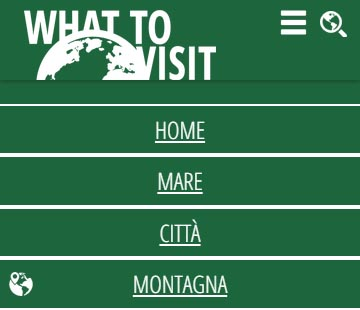
\includegraphics[height=4.65cm,width=5.4cm]{images/pres_nav_m.jpg}
                \caption{Dispositivi mobili}
                \label{fig:Nav-mobile}
        \end{subfigure}
        \caption{I menù di navigazione di WTV}\label{fig:Display-Nav}
\end{figure}

\subsubsection{Searchbar}\label{sec:Pres-Searchbar}
La \textbf{searchbar} è un elemento presente in \textit{tutte le pagine del
sito} e, nonostante possa trovarsi in posizioni diverse, nell'\textbf{header}
per l'\textit{homepage} e nella \textbf{breadcrumb} nelle \textit{pagine di II
e III livello}, essa sarà sempre riconoscibile in quanto, oltre ad essere
l'unica casella di testo con sfondo bianco, il testo sarà verde scuro e
sopratutto il \textit{submit-botton} sarà rappresentato da una lente
d'ingrandimento, immagine spesso usata nel web per indicare la ricerca, che
verrà posta a destra della casella.

Questo elemento non viene visualizzato in maniera completamente diversa a
seconda del foglio di stile, eccezion fatta per il foglio \texttt{playout.css}
(Vedi punto \ref{sec:presentazione}) che elimina dalla stampa tale elemento in
quanto in quanto ritenuto non rilevante nel caso l'utente voglia stampare
informazioni su località o pagine secondarie.
Nelle visualizzazioni per \textbf{Screen} e per \textbf{Dispositivi mobili},
la searchbar si differenzia solamente per la posizione del
\textit{submit-botton}, posto a destra nella versione \textbf{Screen} ed a
sinistra in quella per \textbf{Dispositivi Mobili}.

\subsubsection{Footer}\label{sec:Pres-Footer}
Il \textbf{footer}, elemento con \texttt{background-color}: verde scuro, è
presente in tutte le pagine del sito. I link di questo box si comportano come
quelli del \textbf{navigation menù} (vedi \ref{sec:Pres-Nav}), sono quindi
sempre bianchi e non fanno distinzione tra ancora visitata o meno, questo
perchè servono all'utente solo come aiuto nella navigazione. Sebbene non ci
sia differenza tra \textit{visited} e \textit{unvisited}, abbiamo comunque
voluto che al passaggio del cursore ci fosse un cambiamento visivo, operato
tramite l'aumento e la diminutione del bordo inferiore.

Il \textbf{Footer} viene comunque visualizzato in maniera diversa a seconda
del foglio di stile utilizzato. La versione \textbf{Screen} e quella
\textbf{Print}, vedranno l'elemento svilupparsi orizzontalmente, occupando
tutta la larghezza della finestra, mentre nel caso di visualizzazione su
\textbf{Dispositivi mobili}, esso si svilupperà in verticale e i link puntati
cursore, si distingueranno per la presenza o meno della sottolineatura.

Un piccolo appunto sul \textbf{footer} riguarda la classe \texttt{foothome}
che, nella versione \textbf{Screen}, discrimina alcune pagine portando
l'elemento direttamente a piè pagina, utilizzando l'attributo
\texttt{position: absolute}.
\begin{figure}[h!]
        \centering
        \begin{subfigure}[b]{0.3\textwidth}
                
\includegraphics[height=0.62cm,width=6cm]{images/pres_footer.jpg}
                \caption{Screen}
                \label{fig:Footer-screen}
        \end{subfigure}
        \hspace{4cm}
        \begin{subfigure}[b]{0.3\textwidth}
                
\includegraphics[height=2.25cm,width=5.4cm]{images/pres_footer_m.jpg}
                \caption{Dispositivi mobili}
                \label{fig:Footer-mobile}
        \end{subfigure}
        \caption{I footer di WTV}\label{fig:Display-Footer}
\end{figure}

\subsection{Il layout delle pagine di I livello}\label{sec:Pres-Iliv}
Di come sono costruite le pagine, si è già parlato nella sezione
\ref{sec:struttura}, ora parliamo invece di come e cosa l'utente deve vedere
nelle pagine del nostro sito.
Nel web le cose non si vedono solo con gli occhi, ma anche con le orecchie e
magari anche con le mani; le scelte che abbiamo effettuato cercano quindi di
venire incontro alle esigenze di tutti, che utilizzino dispositivi con
dimensioni di schermo ridotte o che utilizzino screen-reader, abbiamo quindi
voluto nascondere elementi in alcune occasioni per poterli utilizzare da altre
parti, oppure abbiamo mostrato cose in un occasione ed in un altra abbiamo
fatto finta di niente.

Partiamo subito quindi parlando della nostra \textit{homepage}, l'unica pagina
di I livello e l'unica con un layout diverso dalle altre. I tre pannelli
centrali vogliono mettere il visitatore davanti ad un bivio, offrendogli però
un riscontro visivo su dove lo porterà un click su uno dei 3 box. Al
passaggio del cursore, ecco che l'immagine di sfondo aumenterà gradualmente la
sua grandezza richiamando a se l'occhio dell'utente per poi tornare
bruscamente alla sua naturale grandezza in caso il cursore vada altrove. Nel
caso in cui CSS3 non fosse supportato dal browser dell'utente, ciò non
comporterebbe disagio poiché l'immagine verrebbe istantaneamente ingrandita,
permettendo al visitatore di comprendere che sta per scegliere la categoria
sopra la quale ha fatto scorrere il mouse.

Oltre ai 3 box, cliccabili su tutta la superfice e non solo sulla parte verde
contentente il nome della categoria, nella \textit{homepage} sono presenti
\textbf{header}, contenente una \textbf{searchbar} più grande di quella delle
altre pagine, ed un \textbf{footer}, elementi già descritti in precedenza nei
paragrafi \ref{sec:Pres-Header}, \ref{sec:Pres-Searchbar} e
\ref{sec:Pres-Footer} e che, come accade per i 3 \textit{homepanel}, si
sviluppano in verticale anziché orizzontalmente.
\begin{figure}[h!]
        \centering
        \begin{subfigure}[b]{0.3\textwidth}
                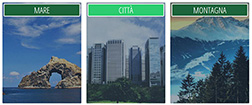
\includegraphics[height=3.7cm,width=8.9cm]{images/pres_home.jpg}
                \caption{Screen}
                \label{fig:Home-screen}
        \end{subfigure}
        \hspace{5cm}
        \begin{subfigure}[b]{0.3\textwidth}
                
\includegraphics[height=8.43cm,width=5.4cm]{images/pres_home_m.jpg}
                \caption{Dispositivi mobili}
                \label{fig:Home-mobile}
        \end{subfigure}
        \caption{La homepage di WTV}\label{fig:Display-Home}
\end{figure}

\subsection{Il layout delle pagine di II livello}\label{sec:Pres-IIliv}
Le pagine di secondo livello, che siano primarie o sencodarie, hanno tutte una
struttura simile così come il layout, in maniera da non creare problemi
all'utente durante la navigazione, utente che potrà però sempre contare sulla
presenza fissa di \textbf{navigation menù}, \textbf{breadcrumb},
\textbf{header} e \textbf{footer}.

Prima di passare a parlare dei due tipi di pagine di II livello, vogliamo
soffermarci sulla \textbf{breadcrumb}, quella barra che molte volte consente
all'utente di capire dove si trova e che, nonostante contenga link utili alla
navigazione, come quelli di \textbf{navigation menù} e \textbf{footer}, vede
colorare le sue ancore di verde scuro e chiaro. I colori dei link, così come
il colore di sfondo di questa barra, sono diversi da quelli del resto del sito
poichè, se per il \textit{background-color} abbiamo optato per un colore molto
simile a quello di sfondo, in quanto non abbiamo ritenuto fosse sempre
importante segnalare all'utente la posizione di questo elemento, abbiamo
voluto fare diversamente con i colori dei link visto che solitamente la
\textbf{breadcrumb}, come suggerisce il nome stesso, serve a ritrovare la
strada ed a capire dove ci si trova focalizzando così la propria attenzione su
cosa c'era prima del passo appena effettuato.

\subsubsection{Il layout delle categorie}\label{sec:Pres-IIliv-cat}
Non appena un utente entra in una delle 3 pagine riguardanti le categorie di
località, il suo occhio verrà catturato dalle immagini di tutti i luoghi
presenti in quella famiglia.

Che la pagina sia visualizzata su \textbf{Dispositivi mobili} o in versione
\textbf{Screen} non cambia, l'utente è portato a focalizzare la propria
attenzione sulla lista di località che alterna immagini del luogo al nome di
esso. Non fa molta differenza quindi se la geolocalizzazione sia attiva o
meno, in quanto è solo un'aggiunta a quello che è il vero contenuto della
pagina, non importa se essa ci fornisce anche una lista delle località più
vicine a noi, perchè ciò che conta è il contenuto, ragion per cui essa non
verrà visualizzata sui \textbf{Dispositivi mobili}.

\subsubsection{Il layout delle pagine secondarie}\label{sec:Pres-IIliv-sec}
Da una parte il \textbf{menù di navigazione} e dall'altra il contenuto, anche
nelle pagine secondarie quindi l'utente potrà concentrarsi su ciò che davvero
gli interessa, ed è proprio per questo che abbiamo deciso che tutti i link
all'interno del contenuto dovessero risaltare ancora di più: da qui la scelta
di scrivere in \textit{grassetto} tutte le porzioni di testo contenute nei tag
\textbf{a}.

Nella visualizzazione di queste pagine su \textbf{Dispositivi mobili}, non
abbiamo voluto forzare la visualizzazione portando a piè pagina il
\textbf{footer}, così come nel caso di una stampa, non abbiamo voluto inserire
elementi non necessari, rendendo così stampabili solamente \textbf{header},
la \textbf{breadcrumb}, in particolare il percorso che faciliterà l'utente nel
caso volesse cercare di nuovo la pagina sul sito, ed il contenuto.

\subsubsection{Il layout Screen e Print}\label{sec:Pres-IIliv-screenPrint}
La differenza tra layout \textbf{Screen} e quello per \textbf{Dispositivi
mobili} sta nel come viene sfruttato ed occupato orizzontalmente lo spazio a
propria disposizione.
Quando l'utente guarda la pagina di una località con una finestra di
dimensione più larga di 780px, potrà notare a sinistra il \textbf{menù di
navigazione}, in centro il contenuto ed a destra.

\subsection{Il layout delle pagine di III livello}\label{sec:Pres-IIIliv}
Il III livello di pagine è quello più importante ed è quello che più cambia il
suo modo di essere visualizzato a seconda del dispositivo utilizzato.
In tutti i casi però abbiamo deciso di rendere visualizzabili il contenuto che
descrive la località e le informazioni schematiche allegate ad essa, compresa
posizione geografica, fornita grazie alla geolocalizzazione, e link utili che
nonostante conducano l'utente fuori dal nostro sito, gli permettono di
ottenere ancora più informazioni riguardo alla località su cui si stava
informando, tutto questo contrassegnado queste ancore con appositi
accorgimenti grafici.

\subsubsection{Il layout Screen e Print}\label{sec:Pres-IIIliv-Screen}
La differenza tra layout \textbf{Screen} e quello per \textbf{Dispositivi
mobili} sta nel come viene sfruttato ed occupato orizzontalmente lo spazio a
propria disposizione.

Quando l'utente guarda la pagina di una località con una finestra di
dimensione più larga di 780px, potrà notare a \textit{sinistra} il
\textbf{menù di navigazione}, al \textit{centro} il contenuto descrittivo
della località ed a \textit{destra} noterà il box di cui si parlava in
precedenza, quello con le informazioni ed i link utili inerenti a quella
località.

Questo tipo di layout punta ad occupare la finestra in tutta la sua larghezza,
offrendo così spazio a nuove soluzioni per quanto riguarda la disposizione del
testo all'interno del box centrale. In particolar modo si è deciso di mettere
come \textit{primo elemento} un immagine significativa che presenti la
località, seguita dal suo nome ed affiancata da un box che ne identifichi la
categoria.

Successivamente inizia la parte descrittiva, divisa in paragrafi ai quali è
sempre associata un immagine. La struttura del blocco centrale ci ha permesso
quindi di poter posizionare a \textit{sinistra} un immagine ed a
\textit{destra} un paragrafo ad essa associato, creando così un effetto lista
che, se associato ad un testo non particolarmente lungo e verboso, renderà
scorrevole la lettura facendo si che il sito ne tragga vantaggio.

Una volta terminata la lettura del testo su quella determinata località, ecco
che il visitatore si troverà, nel caso supporti la funzione, di fronte alla
sezione commenti, potendo così visualizzare o postare commenti su quel luogo.
La visualizzazione dei commenti viene fatta a gruppi, evitando così che
l'utente si ritrovi da un momento all'altro a vede comparire decine e decine
di recensioni. La grafica di ogni singolo commento pone in risalto la data di
pubblicazione, inserita in un apposito span con \texttt{background-color}:
verde chiaro affiancato dal nome dell'utente che ha scritto la recensione.

\subsubsection{Il layout su Dispositivi mobili}\label{sec:Pres-IIIliv-Mobile}
A differenza di quel che accade per il layout \textbf{Screen}, la descrizione
della località non è affiancata, bensì seguita, dal box con le informazioni ed
i link utili su quel luogo. Un altra differenza riguardante la visualizzazione
delle pagine di III livello su \textbf{Dispositivi mobili}, è l'alternarsi di
testo e figure, già a partite dall'immagine di presenzazione; in questo layout
infatti troveremo prima il titolo del paragrafo, poi l'immagine e
successivamente il testo.

Sempre parlando di immagini, arriviamo a discutere della differenza
fondamentale tra il layout per cellulari e quello per dispositivi con
larghezza di schermo compresa tra i 480 ed i 780px:
\begin{itemize}
\item Nel caso di dispositivi con schermo di larghezza inferiore ai 480px,
l'immagine sarà larga il 100\% della grandezza del dispositivo;
\item Nel caso di finestre con larghezza superiore a 780px, ecco che la figura
occuperà il 60\% della larghezza della finestra, questo accade sia per le
immagini dei paragrafi, sia per quelle delle liste di definizioni. Questa
distinzione è atta a far si che l'utente possa comunque godere delle immagini
messe a sua disposizione, perchè trattandosi di un sito che ha lo scopo di
introdurre al visitatore nuove località, ecco che un minimo di qualità, e
purtroppo anche di peso, è più che dovuta.
\end{itemize}

\begin{figure}[h!]
        \centering
        \begin{subfigure}[b]{0.3\textwidth}
                
\includegraphics[scale=0.7]{images/pres_descr.jpg}
                \subcaption{Screen}
                \label{fig:Descr-screen}
        \end{subfigure}
        \hspace{5cm}
        \begin{subfigure}[b]{0.3\textwidth}
                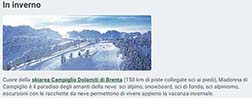
\includegraphics[scale=0.7]{images/pres_descr_t.jpg}
                \subcaption{Tablet}
                \label{fig:Descr-tablet}
        \end{subfigure}
        \begin{subfigure}[b]{0.3\textwidth}
                \centering
                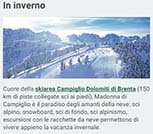
\includegraphics[scale=0.7]{images/pres_descr_m.jpg}
                \subcaption{Mobile}
                \label{fig:Descr-mobile}
        \end{subfigure}
        \caption{Come viene visto il testo su WTV}\label{fig:Display-Descrloc}
\end{figure}

\subsection{Considerazioni finali sui fogli di stile applicati}\label{sec:Pres-CSSValid}
All'interno di ogni pagina, in \textit{basso a destra}, troverete un immagine
che indica che il nostro sito utilizza CSS valido, ma sopratutto ci teniamo a
sottolineare che abbiamo cercato di non abusare di tecnologie, quali CSS3, non
supportate da tutti i browser, creando quindi dei meccanismi che potessero in
ogni caso portare l'utente a vivere al meglio l'esperienza What To Visit.

Terminiamo questa sezione parlando quindi di come abbiamo voluto nascondere
agli occhi di molti alcuni elementi, quali alcune label che quindi non saranno
visibili all'occhio umano, o di come abbiamo cercato di nasconderne altri a
tutti, come accaduto nel caso di layout \textbf{Screen} quando abbiamo
utilizzato la caratteristica \texttt{display: none} per nascondere
completamente il form contenente i \textit{trigger} utilizzati successivamente
nei layout per \textbf{Dispositivi mobili}.
 % IN PROGRESS

\section{Front-end}
Gli script introdotti per la parte front-end, interamente sviluppata in
\textbf{JavaScript}, offrono funzionalità che permettono una migliore
esperienza per l'utente.


Nello specifico sono state inserite le seguenti features:
\begin{itemize}
\item un cookie per il salvataggio del nome utente al momento della
pubblicazione di un nuovo commento;
\item il placeholder nella barra di ricerca località;
\item uno script relativo ai commenti utente che si occupa di controllare,
caricare e nascondere i dati inseriti nella form di pubblicazione;
\item un modulo che effettua la geolocalizzazione.
\end{itemize} 
Per ogni caratteristica sopra elencata si è cercato di separare il codice nel
modo più chiaro possibile; a tal fine si è scelto di utilizzare la libreria
require.js (\texttt{http://requirejs.org}) che si occupa essenzialmente di
caricare files situati in percorsi diversi modularizzando quindi i vari
script.

Require.js si è dimostrato un valido \textit{module loader} anche per la sua
estesa compatibilità con i browser (IE 6+, Firefox 2+, Safari 3.2+, Chrome
3+, Opera 10+).

Nello script \texttt{main.js} sono presenti delle variabili globali; tuttavia,
queste vengono inizializzate ed utilizzate solo quando ciò è sia possibile che
necessario (ad esempio una variabile relativa ad un elemento presente solo
nelle pagine di terzo livello non viene inizializzata al caricamento della
homepage).

\subsection{Gestione cookie}
Per immagazzinare persistentemente la username dell'utente abbiamo deciso di
creare un cookie.

Lo scopo di questo è velocizzare la compilazione di un commento; infatti,
l'utilizzatore, avendo pubblicato una prima volta, alla sua seconda troverà
già riempito il campo nome utente.

Nei nostri script sono state implementate una funzione per l'inizializzazione
ed una per il recupero/lettura del cookie appena creato.

In fase di creazione del cookie, oltre alla coppia chiave-valore abbiamo
aggiunto come terzo parametro una data di scadenza impostata a 15 giorni.
La funzione di recupero restituisce il valore del cookie se questo è presente,
successivamente il valore verrà inserito nel documento HTML e l'utente vedrà
la username già compilata.

\subsection{Inserimento placeholder in barra di ricerca}

Poichè il nostro progetto è conforme allo standard XHTML 1.0 Strict ed  il tag
\textit{placeholder} non vi è definito, abbiamo dovuto usare una funzione
JavaScript per riuscire nel nostro intento di includerlo.


Si è quindi deciso di collegare la gestione degli eventi \textit{onBlur()} e
\textit{onFocus()} a due funzioni definite nello script \texttt{main.js}.
Queste due funzioni assicurano un comportamento tale che se la barra di ricerca
non possiede il focus e non contiene testo inserito dall'utente, visualizza un
\textbf{placeholder} ``Nome località" per aiutare l'utente a capire cosa
inserire in quella barra di ricerca, fornendo una classe diversa a questo
testo per enfatizzarla e distinguerla dal testo inserito dall'utente.

Se invece la barra di ricerca acquisisce il focus, vengono aumentate le
dimensioni della stessa, scompare il placeholder (se presente) ma non un
eventuale testo inserito dall'utente. A questo punto l'utente può inserire un
testo, al quale verrà attribuita la classe predefinita prevista per il testo.

Se la barra di ricerca perde il focus, allora questa continuerà a visualizzare
il testo inserito dall'utente oppure verrà nuovamente visualizzato un placeholder (con classe di enfasi), nel caso in cui l'utente non avesse inserito testo.


\subsection{Gestione dei commenti}
Nelle pagine delle località (sezione \ref{sec:struttLoc}) sono stati
inseriti dei pulsanti per visualizzare, nascondere e pubblicare commenti; qui
di seguito viene descritto il modo con cui queste tre operazioni
(visualizzazione, rendere invisibili e pubblicazione dei commenti) sono state
gestite sul lato client di What To Visit.

\subsubsection{Visualizzazione commenti}\label{sec:visComm}
I commenti sono visibili per tutti i browser fuorchè Internet Explorer, nel
cui caso viene mostrato un messaggio di scuse all'utente per la mancanza della
funzionalità.

Questo è dovuto al fatto che i commenti non sono già presenti nella pagina al
momento del caricamento, ma vengono importati da un file XML e quindi
trasformati tramite un foglio di stile XSLT, che trasforma i commenti in liste
prive di ordine i commenti presenti nel file; in particolare:
\begin{itemize}
\item lo script che applicava il foglio di stile XSLT al file XML forniva
degli output parziali e incompleti utilizzando la funzione prevista per
Internet Explorer, mentre la funzione supportata da tutti gli altri browser
forniva un frammento di documento facilmente manipolabile;
\item il risultato fornito dalla funzione prevista per IE non riusciva ad
essere gestito come elemento nodo ma solamente come stringa, mentre con
la funzione supportata da tutti gli altri browser veniva prodotto un elemento
di tipo nodo sul quale era possibile ricercare tra i nodi figli la lista
contenente i commenti relativi solamente alla località della pagina.
\end{itemize}

Se non vi sono commenti da visualizzare viene visualizzata la stringa
``Non vi sono commenti da visualizzare", altrimenti i commenti vengono
visualizzati a gruppi di due ad ogni pressione del pulsante
``Visualizza commenti" fin tanto che ci sono commenti; la divisione di
documento contenente i commenti viene creata ed allocata nel documento solo
alla prima pressione del pulsante ``Visualizza commenti".

I pulsanti ``Visualizza commenti" può essere in tre stati e questi vengono
assegnati via JavaScript tramite delle classi:
\begin{itemize}
\item \texttt{com-runnable}: non sono visualizzati commenti e si può
richiedere la loro visualizzazione (se l'utente sta usando
Internet Explorer o se non vi sono commenti, solo in seguito alla pressione
del pulsante sarà avvisato dell'impossibilità di mostrargli dei commenti sulla
località)
\item \texttt{com-running}: sono attualmente visualizzati alcuni commenti ma è
possibile visualizzarne altri
\item \texttt{com-notrunnable}: non sono presenti ulteriori commenti da
visualizzare
\end{itemize}

\subsubsection{Rendere invisibili i commenti}
Dopo aver visualizzato tutti i commenti di una località o parte di questi,
l'utente ha la possibilità di nasconderli tramite la semplice pressione di un
pulsante.

Ciò è stato realizzato collegando l'evento onclick del pulsante
``Nascondi commenti" ad una funzione \texttt{nascondi\_c()}, che toglie i
commenti presenti nella divisione in cui erano visualizzati e pone il pulsante
``Visualizza commenti" nello stato \texttt{com-runnable} se erano presenti
commenti.

Il pulsante ``Nascondi commenti" può essere in due stati, assegnati anch'essi
attribuendo delle classi al pulsante:
\begin{itemize}
\item \texttt{com-runnable}: sono visualizzati commenti e si offre all'utente
la possibilità di nasconderli
\item \texttt{com-notrunnable}: non sono visualizzati commenti, perciò per non
creare confusione all'utente si segnala che il pulsante è inutilizzabile
(un'eventuale pressione di questo non produrrebbe alcun output visibile)
\end{itemize}


\subsubsection{Pubblicazione dei commenti}
Nel sito è prevista per gli utenti la possibilità di inserire un proprio commento
inerentemente ad una determinata località. A questo scopo, al termine della sezione 
della pagina dedicata alla visualizzazione dei commenti, vi è il pulsante 
``Pubblica il tuo commento" che permette di visualizzare un form per l'inserimento. 
Tale pulsante può trovarsi in due stati:
\begin{itemize}
\item Disattivo: il form non viene visualizzato
\item Attivo: il pulsante è stato attivato dall'utente causando
quindi la visualizzazione del form per l'inserimento.
\end{itemize}

Il form ha inizialmente, quando disattivo, una classe \texttt{class="hidden"} 
che viene gestita in CSS per nasconderlo. Nel momento in cui l'utente attiva il pulsante
``Pubblica il tuo commento" il codice JavaScript si occupa di modificare tale classe
eliminandone il valore. In questo modo il form compare permettendo all'utente
di inserire il proprio commento. 
Il form è costituito da due campi e due pulsanti così caratterizzati:
\begin{itemize}
\item \textbf{Username:} campo in cui viene richiesto uno username di identificazione
eventualmente compilato automanicamente tramite il valore del cookie precedentemente creato
\item \textbf{Testo del commento:} campo in cui l'utente può inserire il testo del proprio commento
\item \textbf{Pubblica:} pulsante la cui attivazione determina l'invio del commento
\item \textbf{Annulla:}  pulsante la cui attivazione determina l'annullamento dell'operazione
\end{itemize}
A ciascuno dei campi sono associate una o più funzioni che si occupano di controllare i dati
in input. E' prevista infatti l'obbligatorietà di inserire un valore per ognuno dei campi 
\textbf{Username} e \textbf{Testo del commento}. Alla perdita del focus dei campi, se il loro contenuto è vuoto, vengono visualizzati i relativi messaggi di errore.
Il pulsante \textbf{Pubblica} si occupa di attivare il codice Perl che esegue l'effettivo
inserimento del commento all'interno dell'apposito file XML. Il pulsante \textbf{Annulla} invece permette all'utente di annullare l'operazione di pubblicazione del proprio commento.
Lo script ad esso associato, dopo aver eliminato il contenuto dei campi, nasconde il form e
annulla l'operazione.

\subsection{Geolocalizzazione}
In questo progetto abbiamo inoltre deciso di implementare un modulo che fa uso
delle API HTML5 per la geolocalizzazione. L'introduzione di tale
caratteristica ha il puro scopo di migliorare la qualità del sito; in assenza
di questa, l'utente avrà comunque accesso a tutte le funzionalità di base.
\begin{flushleft}
Grazie al modulo in questione, dopo aver acconsentito a fornire i dati sulla
propria posizione e a seconda della pagina in cui si trova, all'utente
verranno mostrate diverse informazioni.
\end{flushleft}

\begin{flushleft}
In particolare, spostandosi sulle pagine ``\texttt{mare.html}" o
``\texttt{citta.html}" oppure ``\texttt{montagna.html}" verranno visualizzate:
\begin{itemize}
\item\textit{una mappa a livello stradale avente tanti marker quante sono le località recensite all'interno della sezione appena raggiunta ed il marker che segnala la posizione attuale;
\item una descrizione recante per ognuna delle località della sezione, la distanza in km dalla posizione attuale.}
\end{itemize}
\end{flushleft}
\begin{flushleft}
In alternativa, spostandosi sulle pagine delle località recensite (es: “praga.html”) verranno visualizzate:
\end{flushleft}
\begin{itemize}
\item\textit{una mappa a livello stradale ad un livello di zoom maggiore rispetto al precedente ed un solo marker posizionato nel centro della città considerata;
\item una piccola descrizione che informa sulla distanza tra la città considerata e la posizione attuale.}
\end{itemize}
È stato scelto di utilizzare Google Maps poiché gli utenti hanno una maggiore
familiarità con le mappe offerte da Google\footnote{ Fonte: comScore Mobile
Metrix, analisi effettuata negli Stati Uniti a Giugno 2014.}, per la qualità
della documentazione relativa alle API offerta da Google e perchè l'utente con
queste mappe riesce facilmente a spostarsi, aumentare il dettaglio di zoom
oppure passare in modalità StreetView in modo semplice ed immediato.

\subsubsection{L'implementazione del modulo in dettaglio}

Vi è un unico script che viene inizializzato al caricamento della pagina ed è
valido sia per le pagine di sezione, (es: ``\texttt{mare.html}") sia per le
pagine delle località turistiche (es: ``\texttt{praga.html}").
Questo è stato possibile attraverso la ricerca di un id presente solamente
nelle pagine relative alle categorie, ma assente nelle pagine delle località.
In tal modo lo script è in grado di discriminare se la pagina è di una
categoria o di una località.

\begin{flushleft}
Per ottenere i dati voluti abbiamo dovuto realizzare una base-dati con le informazioni delle località recensite attraverso un oggetto JSON così formato:
\end{flushleft}
\begin{verbatim}
   var località = {
       "Parigi": {
	          "name": "Parigi",
	          "loc":"Città",
	          "lat": 48.856614,
	          "lon":  2.3522219
       },
       //...
   }
\end{verbatim}
\begin{flushleft}
La funzione principale dalla quale estrapoliamo poi tutti i dati è
\textit{getLocation()}.

Invocando questa funzione viene innanzitutto verificato se il browser supporta
la geolocalizzazione, fornendo un messaggio di errore nel caso in cui non la
supportasse; se invece il browser supporta questa funzionalità, viene chiamata
la funzione \textit{navigator.geolocation.getCurrentPosition(showPosition}) la
quale recupera latitudine e longitudine della posizione attuale del
dispositivo utilizzato dall'utente.
\end{flushleft}
\begin{flushleft}
La funzione \textit{CalcolaDistanza(mylat,mylon,lat,lon)}, come dice il nome, si occupa di calcolare la distanza fra 2 coordinate geografiche; essa prende come argomenti latitudine e longitudine dei due punti desiderati ed attraverso la formula dell'emisenoverso ne restituisce la distanza in km.
\end{flushleft}

\begin{flushleft}
La funzione \textit{showPosition(position)} ha lo scopo di creare l'interfaccia per i dati ed è infatti la funzione più corposa dello script; essa effettua :
\end{flushleft}
\begin{itemize}
\item l'inizializzazione e successivamente la collocazione  della mappa con i marker nel documento HTML;
\item il filtraggio delle sole località da considerare;
\item il riordinamento per distanza minore dalla posizione attuale delle località nelle pagine di sezione;
\item la creazione e la collocazione degli elementi html che costituiscono le informazioni di distanza.
\end{itemize}



















 % 90%

\section{Back-end}
Per quanto riguarda la programmazione lato server, il sito \textit{What To
Visit} offre due funzionalità: con la prima l'utente può inserire commenti,
mentre con la seconda si permette all'utente di accedere alla pagina di una
località tramite una searchbar.

\subsection{Inserimento commenti}
Dal momento che il sito offre la funzionalità di visualizzare commenti inseriti
dagli utenti, questi devono essere salvati in uno o più file nel server. Più
precisamente, ogni commento viene salvato in un file XML chiamato
\texttt{commenti.xml} presente nel server.
Questo documento, valido rispetto allo schema \texttt{commenti.xsd}
(progettato seguendo il modello "\textit{Tende alla Veneziana}), contiene
delle liste di commenti divisi per località; ogni commento, a sua volta,
possiede un corpo, un utente che l'ha scritto e una data in cui è stato
scritto (nel formato AAAA-MM-GG come anticipato nella sezione
\ref{sec:requisiti}). Naturalmente, all'inizio una località può non avere
alcun commento oppure, se qualche commento dovesse essere rimosso per cause di
forza maggiore (ad esempio illegalità o perchè viola i diritti d'autore di un
individuo, come specificato nella pagina della Normativa della Privacy), un
tag \texttt{localita} può rimanere senza commenti.

Lo script di inserimento commenti è stato scritto in Perl utilizzando la
tecnologia \textbf{CGI} (Common Gateway Interface), in modo da riuscire
facilmente a ottenere i dati passati con la form per inserire un commento
presente nelle pagine delle località.

Successivamente lo script procede utilizzando la libreria \textbf{LibXML}, con
le cui funzionalità legge il file dei commenti e cerca il nodo
\texttt{localita} in cui inserire il commento con una query XPath.
Una volta trovato, viene creato il frammento XML da aggiungere alla lista dei
commenti già presenti per la stessa località. Una volta aggiunto il commento,
lo script scrive la modifica sul file XML e reindirizza l'utente alla pagina
della località in cui ha inserito il commento.

\subsection{Barra di ricerca}
L'utente durante la navigazione nel sito ha a disposizione anche una barra di
ricerca; tramite questa, può scrivere il nome di una località (case
insensitive in lingua italiana o in lingua originale) e venire reindirizzato
direttamente alla pagina della località ricercata; se la ricerca non dovesse
trovare nessun risultato, l'utente deve visualizzare una pagina che lo informi
che la ricerca non è andata a buon fine.

Per ottenere questo risultato, è stato scritto uno script in Perl utilizzando
la tecnologia \textbf{CGI} per acquisire il parametro \texttt{\$place} dove è
presente la richiesta effettuata dall'utente e, in caso di ricerca fallita,
per creare la pagina da far visualizzare all'utente.

Lo script inizialmente confronta la stringa ricevuta in input con delle
alternative prefissate; se la stringa passata corrisponde ad una di queste,
allora l'utente viene reindirizzato alla località cercata con successo.
In caso contrario, si esegue una stampa di una pagina con la sezione
head composta come quella nelle altre pagine, header come nelle pagine
secondarie, breadcrumb, nav con possibilità di andare nelle pagine delle
categorie, corpo (dove si informa l'utente di cosa è successo) e footer.
 % 100%

\section{Accessibilità}\label{sec:accessibilita}
Nel sito non è stato indicato nessuno standard di accessibilità raggiunto.
Tramite un analisi, si è notato inoltre che non vengono soddisfatte nè le
richieste di WAI-A WCAG2.0 nè della ``section 508".
Di seguito verranno infatti descritte le mancanze rilevate nel sito in termini
di accessibilità, ordinate secondo le 14 linee guida di WAI; dove non conforme,
verrà indicato la priorità del punto di controllo dove è stata riscontrata la
mancanza.

\subsection{Linee guida per l'accessibilità}

\subsubsection{Fornire alternative equivalenti al contenuto audio e visivo}
\begin{enumerate}
\item Non sempre viene fornito un equivalente testuale per gli elementi non
testuali, ad esempio nella pagina principale mancano gli attributi \texttt{alt}
ai tag \texttt{img}
(\textit{Priorità 1});
\item Non sono presenti mappe immagine, perciò 1.2 è rispettato;
\item Non sono presenti filmati, perciò 1.3 è rispettato;
\item Non sono presenti filmati, perciò 1.4 è rispettato;
\item Non sono presenti mappe immagine, perciò 1.5 è rispettato.
\end{enumerate}

Il punto di controllo 1.1 fallisce e questo è sufficiente per dire che la
pagina non è accessibile per WAI-A WCAG2.0. Di seguito non verrà più
evidenziato tale fatto (nemmeno per i gradi successivi di accessibilità) poichè
il non-rispetto di un solo punto di controllo compromette il grado complessivo
di accessibilità del sito.

\subsubsection{Non fare affidamento sul solo colore}
\begin{enumerate}
\item L'informazione arriva tramite indicazioni indipendenti dal colore;
\item Il contrasto è abbastanza marcato da poter permettere una corretta visualizzazione del sito e, anche nel caso di mancanto caricamento delle immagini di sfondo, sono stati utilizzati degli accorgimenti che garantiscono una visualizzazione decente di alcuni elementi come i titoli/intestazioni.
\end{enumerate}

\subsubsection{Usare marcatori e fogli di stile e farlo in modo appropriato}
\begin{enumerate}
\item Le pagine sono scritte secondo lo standard \textbf{XHTML 1.0 Strict},
sebbene poi non sempre venga rispettato;
\item Tutte le pagine si riferiscono correttamente allo schema \textbf{DTD} di
XHTML 1.0 Strict;
\item Il tag \textit{hr} è utilizzato per meri scopi presentazionali, ovvero
l'inserire un bordo tra delle intestazioni e il contenuto sottostante (ad
esempio in \texttt{about.html}); oltre a questo, sono talvolta inseriti
\texttt{span} per puro scopo presentazionale e non semantico, come quello in
\texttt{\#path} (\textit{Priorità 2});
\item Vengono utilizzate delle unità assolute come \texttt{font-size: medium}
per il testo (\textit{Priorità 2});
\item Gli elementi di intestazione sono usati correttamente, tuttavia si
potrebbe pensare di inserirne altri per favorire la lettura del contenuto da
parte di screen-reader o altri dispositivi che fanno molto affidamento sulle
intestazioni;
\item Vi sono alcune \texttt{dl} che vengono scritte però marcate come
\texttt{ul}, comportando l'aggiunta di tag come \texttt{strong} a parti
dell'item listato per emulare i tag \texttt{dt} e \texttt{dd}
(\textit{Priorità 2});
\item Non sono presenti citazioni, perciò 3.7 è rispettato.
\end{enumerate}

\subsubsection{Chiarire l'uso di linguaggi naturali}
\begin{enumerate}
\item Non viene mai segnalato il cambio linguaggio, ad esempio \textit{home} o
\textit{user} in \texttt{accesso.html} (\textit{Priorità 1});
\item Non vengono mai segnalate abbreviazioni, ad esempio \textit{LDV} in
qualsiasi pagina di un libro o ``\textit{J.K. Rowling}" in
\texttt{ricerca.html} (\textit{Priorità 3});
\item Viene correttamente identificato il linguaggio del documento, perciò 4.3
è rispettato.
\end{enumerate}

\subsubsection{Creare tabelle che si trasformino in maniera elegante}
\begin{enumerate}
\item Non sono presenti tabelle, perciò 5.1 è rispettato;
\item Non sono presenti tabelle, perciò 5.2 è rispettato;
\item Non sono presenti tabelle, perciò 5.3 è rispettato;
\item Non sono presenti tabelle, perciò 5.4 è rispettato;
\item Non sono presenti tabelle, perciò 5.5 è rispettato;
\item Non sono presenti tabelle, perciò 5.6 è rispettato.
\end{enumerate}

\subsubsection{Assicurarsi che le pagine che danno spazio a nuove tecnologie
si trasformino in maniera elegante}
\begin{enumerate}
\item Il contenuto, seppur presentando errori di markup, è sufficientemente
leggibile e comprensibile senza fogli di stile, perciò 6.1 si può ritenere
rispettato;
\item Non si ritiene che i contenuti dinamici del sito possano essere
modificati una volta inseriti, se non per i commenti in coda ai libri;
tuttavia l'aggiornamento automatico tramite AJAX o altre tecnologie esulava
dagli obiettivi del corso di Tecnologie Web, perciò 6.2 si può ritenere
rispettato;
\item Le pagine perdono gran parte della loro usabilità disattivando
JavaScript, ad esempio ogni form, anzichè avere un input di tipo
\textbf{submit}, gestisce la sottomissione dei dati inseriti via JavaScript
con un input di tipo \textbf{button}, compromettendo normali operazioni che
sarebbero possibili utilizzando nella struttura i tag semanticamente corretti
(\textit{Priorità 1});
\item I gestori degli eventi non dipendono da particolari dispositivi che
utilizzano JavaScript, perciò 6.4 è rispettato;
\item Le pagine che non risultano accessibili disattivando JavaScript non
forniscono alcuna pagina o presentazione alternativa (\textit{Priorità 2}).
\end{enumerate}

\subsubsection{Assicurarsi che l'utente possa tenere sotto controllo i
cambiamenti di contenuto nel corso del tempo}
\begin{enumerate}
\item Nessun componente nella pagina causa fenomeni di sfarfallio, perciò 7.1
è rispettato;
\item Nessun componente nella pagina causa fenomeni di lampeggiamento, perciò
7.2 è rispettato;
\item Nessun componente nella pagina si muove una volta caricato, perciò 7.3 è
rispettato;
\item Le pagine non si aggiornano automaticamente, perciò 7.4 è rispettato;
\item Non vi sono pagine che effettuano auto-reindirizzamento, perciò 7.5 è
rispettato.
\end{enumerate}

\subsubsection{Assicurare l'accessibilità diretta delle interfacce utente
incorporate}
\begin{enumerate}
\item Gli script sono ritenuti accessibili verso i dispositivi che li
supportano, perciò 8.1 è rispettato.
\end{enumerate}

\subsubsection{Progettare per garantire l'indipendenza da dispositivo}
\begin{enumerate}
\item Non sono presenti mappe immagine, perciò 9.1 è rispettato;
\item Ogni elemento è accessibile indipendemente dal dispositivo con cui si
naviga nel sito, perciò 9.2 è rispettato;
\item Gli eventi si riferiscono a gesture o actions astratte o logiche e non
relative a specifici dispositivi, perciò 9.3 è rispettato;
\item Non è specificato un ordine di tabulazione diverso da quello di default,
sebbene potrebbe essere utile in questo sito (\textit{Priorità 3});
\item Non sono definite scorciatoie da tastiera, il che potrebbe essere
positivo o negativo a seconda delle motivazioni che risiedono dietro questa
scelta; 9.5 si può ritenere rispettato.
\end{enumerate}

\subsubsection{Usare soluzioni provvisorie}
\begin{enumerate}
\item La finestra attiva non viene mai cambiata nè vengono generate nuove
finestre nè appaiono finestre a cascata, perciò 10.1 è rispettato;
\item Sebbene le label degli input nei form siano associate in modo erroneo
(come discusso nella sezione \ref{sec:acc-form}), queste sono posizionate
correttamente a livello presentazionale rispetto ai rispettivi input, perciò
10.2 è rispettato;
\item Non ci sono tabelle, perciò 10.3 è rispettato;
\item I placeholder ci sono, ma non sempre funzionano nel modo aspettato (come
discusso nella sezione \ref{sec:acc-form}) (\textit{Priorità 3});
\item Non sono presenti molti link nelle pagine e nessuno di questi è
adiacente a un altro senza altri elementi o tag tra i due link, perciò 10.5 è
rispettato.
\end{enumerate}

\subsubsection{Usare le tecnologie e le raccomandazioni del W3C}
\begin{enumerate}
\item Vengono utilizzate solamente tecnologie W3C (anche se talvolta non
rispettando gli standard), perciò 11.1 è rispettato;
\item Le label dei form sono associate al contenuto degli attributi
\texttt{name} (come detto nella sezione \ref{sec:acc-form}) e non a quello
degli attributi \texttt{id}, come da raccomandazione W3C; essendo pratica non
prevista dall'ente, presumibilmente è anche disapprovata
(\textit{Priorità 2});
\item Non si vedono nè localizzazione nè globalizzazione come prospettive di
tale sito, perciò 11.3 è rispettato;
\item Durante la realizzazione del sito probabilmente non è stato notato che
le pagine non rispettano gli standard o che presentano problemi di
accessibilità, perciò non sono fornite versioni alternative
\textit{accessibili} delle pagine del sito (\textit{Priorità 1}).
\end{enumerate}

\subsubsection{Fornire informazione per la contestualizzazione e
l'orientamento}
\begin{enumerate}
\item Non sono presenti \textbf{frame}, perciò 12.1 è rispettato;
\item Non sono presenti frame, perciò 12.2 è rispettato;
\item I campi delle form sono raggruppati con tag \texttt{fieldset} e
\texttt{legend}, perciò 12.3 è rispettato;
\item Come descritto nella sezione \ref{sec:acc-form}, i tag \texttt{label}
non sono associati agli input correttamente (\textit{Priorità 2}).
\end{enumerate}

\subsubsection{Fornire chiari meccanismi di navigazione}
\begin{enumerate}
\item I link fanno effettivamente capire dove portano, ma mancano gli
attributi \texttt{title} per spiegare meglio cosa riferisce l'ancora, perciò
13.1 si può ritenere rispettato in modo lasco;
\item L'utilizzo dei meta tag è sempre scorretto, poichè i contenuti dei pochi
tag presenti sembrano presi da un template XHTML (ad esempio in
\texttt{about.html} il tag \texttt{description} ha come contenuto
\textit{Inserisci le descrizioni}) e mancano tag importanti, come
\texttt{author} (\textit{Priorità 2});
\item Non è presente nessuna pagina dedicata all'orientamento sul sito, nè
mappa nè un indice ben definito (non è presente nemmeno una \textit{sitemap}
\footnote{\texttt{https://support.google.com/webmasters/answer/183668?hl=it}}
vera e propria), non rispettando di fatto il punto di controllo 13.3
(\textit{Priorità 2});
\item Come descritto nella sezione \ref{sec:user-ui_consistency}, gli elementi
di navigazione non sono consistenti o coerenti nelle varie pagine del sito
(\textit{Priorità 2});
\item Il sito non dispone sempre di una barra di navigazione, ad esempio nella
pagina visualizzata se si fallisce l'accesso (\textit{Priorità 3});
\item Il sito non ha necessità di forkare codice per diversi
\textit{user agent}, perciò 13.6 è ritenuto rispettato;
\item Il sito offre diversi metodi di ricerca (sebbene questa non funzioni
correttamente come descritto nella sezione \ref{sec:schema-org}), perciò 13.7
è rispettato;
\item In alcune parti l'informazione più significativa non è posta all'inizio
di elenchi, come descritto nella sezione \ref{sec:schema-elenchi}
(\textit{Priorità 3});
\item Non sono presenti documenti composti da più pagine, perciò 13.9 è
rispettato;
\item Non sono presenti immagini realizzate con l'\textit{ASCII multi-line}
\footnote{\texttt{https://trendimpulse.wordpress.com/tag/multiple-lines-ascii-art/}}, perciò 13.10 è rispettato.
\end{enumerate}

\subsubsection{Assicurarsi che i documenti siano chiari e semplici}
\begin{enumerate}
\item Anche se il testo non sempre è grammaticalmente corretto e semplice, si
ritiene che la (\textbf{seconda}) scelta sia dovuta al fatto che l'audience è
un pubblico di cultura letteraria medio-alta (essendo il sito di una
biblioteca), perciò 14.1 si può ritenere rispettato;
\item Sono mostrate le immagini delle copertine dei libri, mentre l'audio
potrebbe essere meno significativo per aumentare il valore del contenuto,
perciò 14.2 è rispettato;
\item Lo stile di presentazione è comune a tutte le pagine, perciò 14.3 è
rispettato.
\end{enumerate}

%%%%%% FINE LINEE GUIDA -> QUI SI METTONO TUTTE LE COSE NON SALTATE FUORI PRIMA

\subsection{Errori non risultati dal confronto con le linee guida}

\subsubsection{Form}\label{sec:acc-form}
I form presentano vari errori:
\begin{itemize}
\item I form sono spesso bizzarramente contrassegnati con la classe
\texttt{forms}, come in \texttt{ricerca.html}, rompendo nuovamente la
separazione presentazione-struttura;
\item Non compaiono gli input di submit, rendendo impossibile la richiesta di
azione di un form se JavaScript è disattivato (si ritiene che non siano stati
messi i submit poichè fosse lievemente più complesso gestire l'arresto
nell'invio della richiesta di sottomissione nel caso in cui i dati inseriti
fossero scorretti, rompendo la separazione comportamento-struttura);
\item Per qualche strano motivo gli input presentano attributi \texttt{name} e
\texttt{id} con contenuto differente;
\item Le label sono associate erroneamente, per cui la pressione sull'elemento
individuato dal tag label non risulta nell'acquisizione del focus sull'input
desiderato;
\item Le ricerche di libri per autore, titolo e collana vengono eseguite con
una chiamata REST di tipo POST, impedendo all'utente di salvare come possibile
segnalibro (una \textbf{boa}, nella \textit{metafora della pesca}) la pagina
contenente i risultati della ricerca effettuata;
\item I placeholder non hanno comportamento del tutto aspettato dall'utente,
dal momento che se l'input perde il focus dopo averlo acquisito ed è vuoto,
non ricompare il placeholder.
\end{itemize}

\subsubsection{Separazione tra elementi del sito}
Qui di seguito vengono evidenziate le incongruenze non precedentemente
segnalate, rispetto alla separazione tra i tre elementi che lo compongono,
ovvero \textbf{struttura}, \textbf{presentazione} e \textbf{comportamento}.

\paragraph{Separazione struttura-comportamento} ~\\
In quasi tutte le pagine HTML c'è codice JavaScript, rompendo in modo netto la
separazione struttura-comportamento.

\paragraph{Separazione struttura-presentazione} ~\\
Alcune classi, come \textit{shiftsx} in \texttt{contatti.html} forniscono
informazioni di carattere presentazionale e non semantico.

Nei form è inserito il tag \texttt{br} a scopo presentazionale, poichè serve
solamente per controllare la posizione del fieldset.

Nella pagina \texttt{registrazione.html} il tag \texttt{br} è usato per far
andare a capo il testo.

Nella pagina \texttt{registrazione.html} è associata la classe
\textit{link\_blok} che presuppone che il link sia visualizzato all'interno di
un proprio blocco, ma ciò non avviene. Il nome della classe non ha carattere
semantico ma presentazionale.

Come in \texttt{generi.html}, sono state inserite classi non necessarie per
modificare l'aspetto presentazionale di elementi (le classi
\textit{adattaicona} associate ai link).

\paragraph{Separazione presentazione-comportamento} ~\\
In \texttt{registration\_control.js}, viene assegnato esplicitamente il colore
di elementi tramite JavaScript (con l'attributo \texttt{style}, inserendo CSS
inline).
 % 80%

\section{Test effettuati} %TODO Graziano, Federica, Carlo i test effettuati da voi
In questa sezione si elencano i test effettuati per ogni prodotto di progetto.
Per i test di accessibilità eseguiti in remoto, il sito è stato caricato su
GitHub Pages.

\subsection{Validazione XHTML}
Ogni pagina è stata validata con il tool offerto da W3C all'indirizzo
\texttt{http://validator.w3.org/\#validate\_by\_input}.

\subsection{Validazione CSS}
Ogni foglio di stile CSS è stato validato con il tool offerto da W3C
all'indirizzo
\texttt{https://jigsaw.w3.org/css-validator/\#validate\_by\_input}.

\subsection{Validazione XML e XSD}
Il file XML dove sono salvati i commenti è stato validato rispetto al suo
schema XSD con il tool offerto da \textit{freeformatter.com} all'indirizzo
\texttt{http://www.freeformatter.com/xml-validator-xsd.html}.

\subsection{Validazione XSLT}
Il file XSLT che permette di trasformare il file XML dove sono salvati i
commenti è stato validato (si è anche verificato il suo corretto
funzionamento) con il tool offerto da \textit{freeformatter.com} all'indirizzo
\texttt{http://www.freeformatter.com/xsl-transformer.html}.

\subsection{JavaScript}
Ogni script JavaScript è stato analizzato tramite il tool di analisi statica di
\textit{WebStorm}, affinchè venissero trovati errori e miglioramenti al codice.

Ogni frammento di codice è stato testato in locale ed in remoto non tralasciando alcun valore nel dominio dei possibili valori in ingresso. Ogni
test è stato effettuato tenendo visibile la \textbf{Javascript Console} del
browser, così da notare eventuali warning o errori nel codice. I test hanno
avuto esito positivo sul prodotto finale.

\subsection{Perl e CGI}
Ciascuno degli script Perl e CGI è stato verificato in locale, con esiti
positivi.

\subsection{Cynthia Says}
Uno dei tool che è stato utilizzato per l'accessibilità delle pagine è Cynthia
Says, inserendo l'URL di ogni pagina caricata su GitHub Pages e richiedendo la
conformità a WCAG 2.0 AAA. Questa scelta è dovuta al fatto che i tentativi per
verificare l'accessibilità di una pagina sono limitati a 10 nell'arco di 24
ore.
Di seguito vengono riportati i risultati ottenuti per \textbf{tutte} le pagine
del sito:

\begin{center}
\begin{tabular}[h!]{ | l | c | }
  \hline
  Conformità & Esito \\
  \hline
  WCAG 2.0 A & Conforme \\
  \hline
  WCAG 2.0 AA & Conforme \\
  \hline
  WCAG 2.0 AAA & Non conforme \\
  \hline
\end{tabular}
\end{center}

Le pagine del sito non sono conformi a WCAG 2.0 AAA poichè:
\begin{enumerate}
\item \textit{Cynthia Says} non riconosceva come pagine di aiuto ``Mappa del
sito" e ``F.A.Q.";
\item il contrasto richiesto per il terzo grado di accessibilità era troppo
elevato per poter garantire una resa grafica piacevole del sito.
\end{enumerate}

\subsection{WAVE}
WAVE (Web Accessibility Evaluation Tool) è uno strumento offerto da
\textit{WebAIM} (WEB Accessibility In Mind) per verificare l'accessibilità
delle pagine. Questo strumento analizza una pagina e fornisce errori,
avvertimenti (warnings), caratteristiche positive, struttura basilare di una
pagina e indicazioni sul contrasto.

Più in particolare, sono stati corretti gli errori trovati (relativi agli
standard 508 e WCAG) non relativi alla lingua delle pagine, dal momento che
nonostante il tag html fosse ben-formato e contenente l'indicazione sulla
lingua utilizzata nella pagina in modo corretto, il sito continuava a
segnalare il falso positivo.

I warnings sono stati corretti solo se effettivamente utili; questo dal
momento che sono stati introdotti volutamente titoli o link ridondanti per
aiutare l'utente a capire dove si trova e che l'uso dei tabindex viene
segnalato come warning, anche se questi sono stati messi per permettere
all'utente di raggiungere subito i link della pagina più rilevanti, saltando
elementi di navigazione o breadcrumb a seconda dei casi.

I contrasti dei colori sono stati regolati per riuscire a superare almeno il
livello di accessibilità WCAG 2.0 AA.

\subsection{Fangs}
\textit{Fangs} è un'estensione per i browser che consente di visualizzare un
sito nello stesso modo in cui verrebbe visualizzato da uno screen reader,
fornendo il testo come sarebbe letto da questo dispositivo, la lista delle
intestazioni e la lista dei link presenti nella pagina.

Sono state controllate tutte le pagine, con esito positivo: le intestazioni
seguono l'ordine logico pensato dai componenti del gruppo, i link sono
visualizzati nell'ordine aspettato e non sono presenti elementi estranei nel
testo corrispondente all'audio che sentirebbe un utente con screen reader,
mentre gli aiuti come il ``salta la navigazione" sono presenti.
 % 80%

%%%%%%%%%%%% B====>
%PER NOI: OGNI SEZIONE CHE AGGIUNGETE BASTA METTERLA NELLA CARTELLA sections
%con un certo nome (facciamo finta che sia pippo.tex) E
%POI AGGIUNGERE QUI SOTTO \include{sections\pippo} COME HO FATTO CON L'ABSTRACT
%%%%%%%%%%%% B====>

%----------------------------------------------------------------------------------------

\newpage % Start the article content on the second page, remove this if you have a longer abstract that goes onto the second page

\end{document}

%%%%%%%%%%% B====>
% Dovete stare attenti ad avere installato texlive-full e texlive-publisher (o nome simile)
% Per compilare, make da terminale nella folder dove è contenuto questo file (ho già fatto io il makefile)
% Prima di committare, make clean e cancellare *.pdf
%%%%%%%%%%% B====>
